%%── PANEL 5: Temas 3, 4 y 5 ─────────────────────────────────────────────────
\panel{LightBg}{%
  \phdr{Emerald}{3 · Coloraci\'on de enteros}
  \begin{tcolorbox}[def,title={$r$-coloraci\'on}]
    {\scriptsize Funci\'on $f:X\to\{1,\ldots,r\}$.
    El conjunto $A$ es \textbf{monocrom\'atico} si $A\subseteq f^{-1}(i)$.}
  \end{tcolorbox}

  \begin{center}
  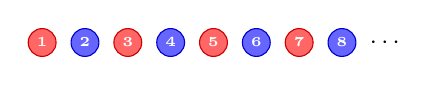
\begin{tikzpicture}[scale=0.68]
    \foreach \n/\c in {1/red,2/blue,3/red,4/blue,5/red,6/blue,7/red,8/blue}{
      \filldraw[\c!60,draw=\c!80!black]
        ({(\n-1)*0.80cm},0) circle (0.26cm);
      \node[text=white,font=\tiny\bfseries] at ({(\n-1)*0.80cm},0) {\n};
    }
    \node[font=\small] at ({8*0.80cm},0) {$\cdots$};
  \end{tikzpicture}
  \end{center}
  {\scriptsize\textbf{Pregunta central:} ?`Toda $r$-coloraci\'on de $\mathbb{N}$
  contiene siempre estructuras aritm\'eticas monocrom\'aticas?}

  \phdr{Navy}{4 · Teorema de Schur (1916)}
  \begin{tcolorbox}[thm,title={Teorema}]
    {\scriptsize Para todo $r\geq 1$ existe $S(r)$ tal que toda
    $r$-coloraci\'on de $\{1,\ldots,n\}$ con $n\geq S(r)$ contiene
    $x,y,z$ monocrom\'aticos con $x+y=z$.}
  \end{tcolorbox}

  \begin{center}
  {\scriptsize\begin{tabular}{lccccc}
  \toprule $r$ & 1 & 2 & 3 & 4 & 5 \\
  \midrule $S(r)$ & 2 & 5 & 14 & 45 & 161 \\
  \bottomrule
  \end{tabular}}
  \end{center}

  \begin{tcolorbox}[ex,title={Consecuencia (Schur)}]
    {\scriptsize Para todo $k$ $\exists\,n$ tal que $\forall$ primo $p>n$,
    $x^k+y^k\equiv z^k\pmod{p}$ tiene soluci\'on no trivial.}
  \end{tcolorbox}

  \phdr{Navy}{5 · Teorema de Van der Waerden (1927)}
  \begin{tcolorbox}[def,title={Progresi\'on aritm\'etica (PA)}]
    {\scriptsize $\{a,\,a+d,\,\ldots,\,a+(k{-}1)d\}$ — tama\~no $k$, raz\'on $d$.}
  \end{tcolorbox}

  \begin{tcolorbox}[thm,title={Teorema}]
    {\scriptsize $\forall\,r,k$ existe $W(r,k)$ tal que toda $r$-coloraci\'on
    de $\{1,\ldots,n\}$ con $n\geq W(r,k)$ contiene una PA monocrom\'atica
    de tama\~no $k$.\\[1pt]
    \textbf{Versi\'on $\infty$:} toda coloraci\'on finita de $\mathbb{Z}^+$
    contiene PA monocrom\'aticas arbitrariamente largas.}
  \end{tcolorbox}

  \begin{center}
  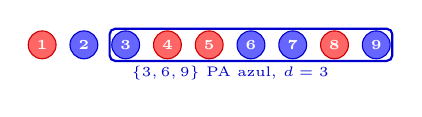
\begin{tikzpicture}[scale=0.68]
    \foreach \n/\c in {1/red,2/blue,3/blue,4/red,5/red,6/blue,7/blue,8/red,9/blue}{
      \filldraw[\c!60,draw=\c!80!black]
        ({(\n-1)*0.78cm},0) circle (0.26cm);
      \node[text=white,font=\tiny\bfseries] at ({(\n-1)*0.78cm},0) {\n};
    }
    \draw[blue!80!black,thick,rounded corners=2pt]
      ({2*0.78-0.30},-0.30) rectangle ({8*0.78+0.30},0.30);
    \node[font=\tiny,blue!80!black] at ({4.5*0.78},-0.52)
      {$\{3,6,9\}$ PA azul, $d=3$};
  \end{tikzpicture}
  \end{center}

  \begin{tcolorbox}[key]
    {\scriptsize\textbf{Cota (Gowers):}
    $W(r,k)\leq 2^{2^{r^{2^{2^{k+9}}}}}$\hfill$W(2,3)=9$\hspace{4pt}$W(2,4)=35$}
  \end{tcolorbox}
}%
